\documentclass[12pt,letterpaper]{ntdhw}


\usepackage{ntdmath}

\title{Project 0: Lisp Introduction and Set Operations}
\author{CSCI 561}

\rhead{Names:}

%\keytrue

\begin{document}
\pagestyle{fancyplain}

\maketitle
\thispagestyle{fancyplain}
%\clearpage

\begin{enumerate}

  \item Describe the Lisp development environment that you used for
  this project.  (\emph{Hint: The correct answer is ALIVE, SLIME, or
    similar.})

    ALIVE

  \item What are the types of the following Lisp expressions?
  \begin{enumerate}
    \item {\tt 1} : \emph{
      An integer Literal.
    }
    \item {\tt (+ 1 2)} : \emph{
      An s-expression that evaluates to an integer (3) because it adds two integers.
    }
    \item {\tt '(+ 1 2)} : \emph{
      A quoted list with three elements that doesn't evaluate.
    }
    \item {\tt (eval '(+ 1 2))} : \emph{
      An s-expression that evaluates to integer (3) because it's evaluating a quoted list with three elements.
    }
    \item {\tt (lambda () (+ 1 2))} : \emph{
      An anonymous function that adds two integers.
    }
    \item {\tt "foo"} : \emph{
      A string literal.
    }
    \item {\tt 'bar} : \emph{
      A quoted symbol bar.
    }
  \end{enumerate}

  \item Tail Calls:
  \begin{enumerate}
    \item What is tail recursion?

    \begin{emph}
      Answer: % Your Answer Here
    \end{emph}

    \item In the recursive implementation, will {\tt fold-left} or
    {\tt fold-right} be more memory-efficient?  Why?

    \begin{emph}
      Answer: % Your Answer Here
    \end{emph}
  \end{enumerate}

  \item Lisp and Python represent code differently.

  \begin{enumerate}
    \item Contrast the representations of Lisp code and Python code.

    \begin{emph}
      Answer: Lisp represents code as lists, allowing it to treat code as data, while Python represents code as text that needs to be parsed before execution.
    \end{emph}

    \item How does Python's {\tt eval()} differ from the approach of Lisp?

    \begin{emph}
      Answer:  Python’s {\tt eval()} evaluates a string of code and it requires parsing, whereas Lisp can directly evaluate lists, since its code is inherently structured as data.
    \end{emph}
  \end{enumerate}

  \item GCC supports an extension to the C language that allows
  local/nested functions (functions contained in other functions).  A
  GCC local function can access local variables from its parent
  function.
  \begin{enumerate}
    \item What problems would arise if you return a function pointer
    to a GCC local function? \emph{(Hint: ``Funarg problem'')}

    \begin{emph}
      Answer: When returning and exiting that scope local variables from the GCC local function's parent function would be deallocated so the returned local function would no longer be able to access them and would produce undefined behaviour.
    \end{emph}

    \item How does Lisp handle this problem?

    \begin{emph}
      Answer: Lisp solves this by packing the function with all the local variables it requires so that no matter where it is used the function will always have access to the environment in which it was created.
    \end{emph}

  \end{enumerate}

  \item Test the performance of your implementation of
    \texttt{merge-sort}.
    \begin{enumerate}

    \item Plot the running time of both your \texttt{merge-sort}
      implementation and the builtin Lisp \texttt{sort} function for
      increasing input sizes.  Include enough data points to
      demonstrate the empirical asymptotic running time.

    \begin{emph}
      \\
      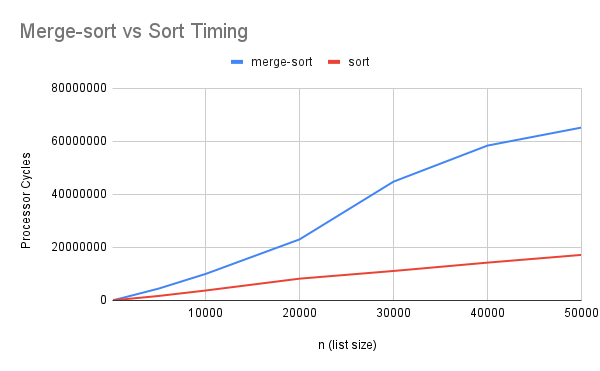
\includegraphics[scale=0.6]{graphics/mergesort1.png} 
      \\
      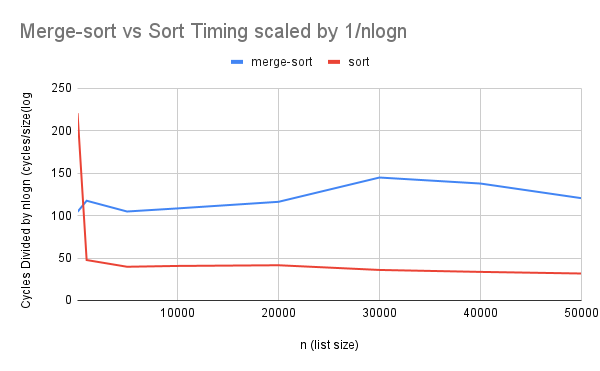
\includegraphics[scale=0.6]{graphics/mergesort2.png}
    \end{emph}

  \item What asymptotic running time did you expect for
    \texttt{merge-sort} and the builtin Lisp \texttt{sort} function, and
    what running time did you observe?  Explain any differences.

    \begin{emph}
      Answer: I expected O(nlogn) time for merge-sort because merge sort takes O(nlogn) time and at no point in my implementation did I use methods with a slower asymptotic time complexity than assumed (such as by splitting a list in O($n^2$) time rather than O(n)). I expected O(nlogn) time for sort because it is a generic sorting algorithm and provided that nothing is known about the list being sorted, O(nlogn) is the best asymptotic running time any existing sorting algorithm can achieve. Both of these hypotheses correlated with the results as shown in the second graph in the previous answer by how dividing the number of cycles by the list size times the log of the list size and plotting that vs the list size creates roughly horizontal lines.
    \end{emph}

    \end{enumerate}

    \item Newton's method is a powerful technique for finding roots of real-valued functions. Given a function \( p(x) \), Newton's method iteratively computes the next approximation \( x_{n+1} \) of the root using its derivative, \( p'(x) \), as follows:

    \[
    x_{n+1} = x_n - \frac{p(x_n)}{p'(x_n)}
    \]

    For this question, you will use your implementation of {\tt find-fixpoint} to find roots of polynomials via Newton's method.
  \begin{enumerate}
    \item Determine \( f(x) \):

    Given a polynomial \( p(x) \) and its derivative \( p'(x) \), determine the function \( f(x) \) that should be used in the {\tt find-fixpoint} function. Write down the expression for \( f(x) \).

    \begin{emph}
      Answer:
      \\ Our {\tt find-fixpoint} function does not have any specific functionality that would prevent it from finding roots if the correct input function was given, thus we need only replace \(f(x) \) with the iterative Newton's expression to find the roots using our function. This means that our function is:
      \[
    f(x) = x - \frac{p(x_n)}{p'(x_n)}
    \]
    \end{emph}

    \item Implement and Test:

    Implement the function \( f(x) \) you derived, and use {\tt find-fixpoint} to find the roots of the following polynomials using Newton's method:
    \begin{enumerate}
      \item \( p(x) = x^2 - 2 \)
      \item \( p(x) = x^3 - x - 2 \)
      \item \( p(x) = x^3 - 6x^2 + 11x - 6 \) (roots are 1, 2, 3)
    \end{enumerate}

    For each polynomial, choose an initial guess and use a precision of \( 0.001 \). Give the parameters to the call to {\tt find-fixpoint} and report the root found by your implementation.

    \begin{emph}
      Answer: % Implement and test, then report the results here.
      \\For \( p(x) = x^2 - 2 \) our function must be: \[
    f(x) = x - \frac{x^2-2}{2x}.
    \]
    \\ We set our initial value as 1.0 to find our positive root and -1.0 to find our negative root. After implementing {\tt find-fixpoint}, we found that the roots were 1.414 and -1.414, respectively.
    \\For \( p(x) = x^3 - x - 2 \), ur function must be: \[
    f(x) = x - \frac{x^3 - x - 2}{3x^2 - 1}.
    \]
  \\ Since there is only one root, we set our initial value as 1.0 to find the root. After implementing {\tt find-fixpoint}, we found the root to be 1.521.
  \\For \( p(x) = x^3 - 6x^2 + 11x - 6 \), our function must be: \[
    f(x) = x - \frac{x^3 - 6x^2 + 11x -6}{3x^2-12x+11}.
    \]
  \\ Since there were three roots, we set our initial values to 0.6, 1.6, and 2.6 to make sure we captured all three roots. After implementing {\tt find-fixpoint} we found the roots to be 1, 2, and 3 respectively.
  \end{emph}

  \end{enumerate}

\end{enumerate}

\end{document}
